\chapter[$\mbox{N}^3$ - A Collection of Datasets for NER and NED in NIF]{$\mbox{N}^3$ - A Collection of Datasets for Named Entity Recognition and Disambiguation in the NLP Interchange Format}
\label{cha:N3}
\graffito{
This chapter presents $\mbox{N}^3$, a collection of three annotated corpora for \ac{NER} and \ac{NED}.,
It has been published in~\cite{n3} and since than build the gold standard for evaluations in papers like \cite{agdistis_iswc, GERBIL}.
The author of this thesis is one of the two main authors, implemented the annotation tool, generated parts of the datasets and co-wrote the paper and its poster. 
}
\lstset{
  basicstyle=\footnotesize\ttfamily,
  breaklines=true,
  captionpos=b,                    % sets the caption-position to bottom
  frame=single,
  %morecomment=[s][\color{blue}]{<}{>},
  morecomment=[s][\color{red}]{"}{"},
  numbers=none  
%  numbersep=5pt,
% numberstyle=\tiny,
%  stringstyle=\tiny
}
%\name{Michael R{\"o}der$^{1,2,\star}$, Ricardo Usbeck$^{1,2,\star}$, Sebastian Hellmann$^{1}$, Daniel Gerber$^1$ \& Andreas Both$^{1,2}$}
%\institute{First Institute Name \email{email address} \and Second Institute Name\thanks{Thank you to...} \email{email address}}
%\address{
%$^{1}$ Agile Knowledge Engineering and Semantic Web, University Leipzig, Germany \\
%$^{2}$ R\,\&\,D, Unister GmbH, Germany}

%\abstract{
%Extracting Linked Data following the Semantic Web principle from unstructured sources has become a key challenge for scientific research. % as well as new business models. \todo{Jens: Which business models? This just appears in the abstract and not the introduction.}
%Named Entity Recognition and Disambiguation are two basic operations in this extraction process.
%%\todo{Jens: maybe "One step towards the realization of ..." - avoid repeating "key driver"} 
%One step towards the realization of the Semantic Web vision and the development of highly accurate tools is the availability of data for validating the quality of processes for Named Entity Recognition and Disambiguation as well as for algorithm tuning.
%This article presents three novel, manually curated and annotated corpora ($\mbox{N}^3$). All of them are based on a free license and stored in the NLP Interchange Format to leverage the Linked Data character of our datasets. %\todoanbo{make more catchy} % for interoperability reasons.
%\\ \newline \Keywords{Datasets, NLP Interchange Format, Named Entity Detection, Named Entity Disambiguation}
%}

%\maketitleabstract

%\section{Introduction}

Automatically extracting and linking Named Entities (NEs) to a particular \ac{KB}  from unstructured, natural language text is an extremely challenging task~\cite{Cucerzan07}. 
Leveraging Linked Data can help developing tools to automatically extract semantic data~\cite{GER+13,AIDA,spotlight,agdistis_iswc}.

The tasks of \ac{NER}  and \ac{NED}  are part of the research area of Information Extraction~\cite{FOX}.
NER is the task of identifying entities of certain types.
%why not use the NERD core classes? 
NED is the task of disambiguating pre-identified named entities towards a certain \ac{KB} .
%NED is based on pre-identified named entities and their disambiguation towards a certain KB. %using various methods.
%RE determines links between entities based on a given context leading to Information Extraction~\cite{fox}.
These IE steps depend on datasets which need human annotation, and therefore make it a time-consuming and expensive task.
%\todo[inline]{Why does RE lead to IE? This formulation seems a little bit strange and does not really fit to the next sentence in which RE is a step of IE.}
%\todo[inline]{Done, but does it really fit in here? (rewrite that section, mention that NED is done by using DBpedia as KB. DBpedia is the central point of the Linked Open Data movement.)}

We present three novel datasets (called $\mbox{N}^3$) in which named entities have been annotated manually. As \ac{KB}  for this annotation we used DBpedia~\cite{dbpedia-swj} which is the central point of the Linked Open Data movement. These datasets have already been used to evaluate~\cite{AIDA,spotlight} as well as in~\cite{GER+13,agdistis_iswc,GERBIL}.
$\mbox{N}^3$ is published using the \ac{NLP} Interchange Format (NIF)~\cite{ISWC2013NIF} ensuring a greater interoperability to overcome the need for corpus-specific parsers. 
The data can be downloaded from the project homepage \url{http://aksw.org/Projects/N3nernednif}.

\todo[inline]{Maybe this section can go to contributions section}
Our main contributions are as follows:
\begin{itemize}
\item The publication of three novel and freely available datasets for \ac{NER} and \ac{NED};
\item An analysis of the underlying corpora;
\item The transformation of these corpora to NIF providing provenance data.
\item Finally, our datasets also allow the analysis of coreference resolution~\cite{NgongaNgomo2014,singh} if the entity is not in the \ac{KB}  of the respective corpus.
\end{itemize}
%\todo[inline]{provide a community based platform (GIT) to improve datasets}
%\todo[inline]{What have we done to get point 5? Do we have that much contributions?}

\section{Corpora}
\label{n3:sec:Features}




In the following section, we present the annotation process as well as specific features for each corpus of the $\mbox{N}^3$-Collection.

During the annotation, we focused on recognizing three main classes of NEs: persons, places and organizations. 
Each identified NE has been manually disambiguated to the DBpedia 3.9  if possible.
In case there was no matching resource from a \ac{KB}  we created an URI\footnote{\url{http://www.w3.org/TR/cooluris/}} using the \url{http://aksw.org/notInWiki/} namespace (see Section~\ref{n3:NIF}).
Additionaly, we resolved coreferences for every named entity, especially, for entities that are not yet in the \ac{KB} . %\todo[inline]{coreference resolved?}

Furthermore, the collection of datasets is annotated by the version and language of the \ac{KB} , hence any change of the underlying database can be analysed.
In order to spread the corpora, we publish them under the Creative Commons BY-NC-SA license\footnote{\url{http://creativecommons.org/licenses/by-nc-sa/4.0/}}.

In general, our corpora contain more documents then any published NIF corpora (\texttt{KORE50} and \texttt{DBpedia Spotlight}) so far.
First order statistics for all datasets, such as the number of documents, words or average word count per document, can be found in Table~\ref{n3:tab:corpus_stats}.
Moreover, Table~\ref{n3:tab:entity_counts} describes the number of entities and URIs known or not known in DBpedia w.r.t. a certain dataset.


\begin{table}[htb!]
	\centering
	\resizebox{\textwidth}{!}{
    \begin{tabular}{lp{0.0cm}cp{0.0cm}D{.}{}{3.0}p{0.0cm}D{.}{}{5.0}p{0.0cm}D{.}{.}{4.2}}
     \toprule
     \textbf{Corpus} && \textbf{Language} && \multicolumn{1}{c}{\textbf{\#Documents}} && \multicolumn{1}{c}{\textbf{\#Words}} && \multicolumn{1}{c}{\textbf{Avg. Words/Doc.}} \\
    \midrule
    News-100 && German && 100 && 48199 && 481.99 \\
	Reuters-128 && English && 128 && 33413 && 261.04 \\
	RSS-500 && English && 500 && 31640 && 63.28 \\
    \midrule
    KORE50 && English && 50 && 1332 && 26.64 \\
    DBpedia Spotlight && English && 10 && 3582 && 358.20 \\
	\bottomrule
	\end{tabular}}
	\caption{Features of the corpora and their documents.}
	\label{n3:tab:corpus_stats}
\end{table}

\begin{table}[htb!]
	\centering
    \begin{tabular}{lp{0.25cm}D{.}{}{4.0}p{0.25cm}D{.}{}{4.0}p{0.25cm}D{.}{}{4.0}p{0.25cm}D{.}{}{4.0}}
     \toprule
	 \multirow{2}{*}{\textbf{Corpus}} && \multicolumn{3}{c}{\textbf{Entities}} && \multicolumn{3}{c}{\textbf{Unique URIs}}\\
	  && \multicolumn{1}{c}{\textbf{DBpedia}} && \multicolumn{1}{c}{\textbf{AKSW}} && \multicolumn{1}{c}{\textbf{DBpedia}} && \multicolumn{1}{c}{\textbf{AKSW}} \\
	\midrule
	News-100 && 1547 && 108 && 315 && 57 \\
	Reuters-128 && 650 && 230 && 299 && 145 \\
	RSS-500 && 524 && 476 && 400 && 449 \\
    \midrule
    KORE50 && 144 && 0 && 127 && 0 \\
    DBpedia Spotlight && 331 && 0 && 249 && 0 \\
	\bottomrule
	\end{tabular}
	\caption{Number of single entities and unique URIs in the corpora.}
	\label{n3:tab:entity_counts}
\end{table}


The distribution of NEs over the texts is shown in Figure \ref{n3:fig:nePerDoc}. 
\begin{figure}[htb!]
  \centering
  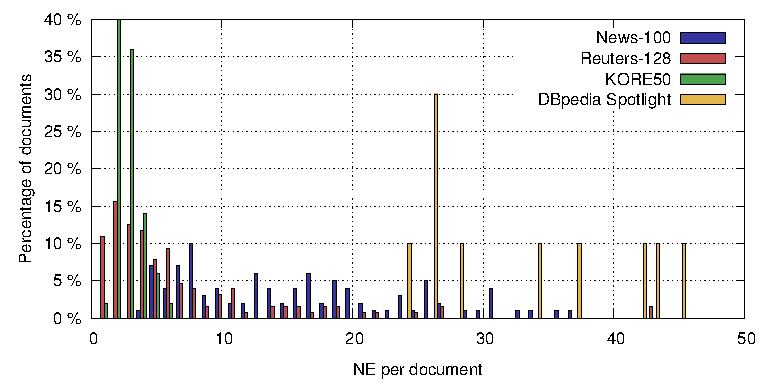
\includegraphics[width=\linewidth]{part_02/benchmarking/LREC_N3NIFNERNED/NE_per_doc.pdf}
  \caption{Distribution of NEs per document. We omitted two outliers from the News-100 corpus containing 55 and 63 NEs.}
  \label{n3:fig:nePerDoc}
\end{figure}

\texttt{RSS-500} has been left out because all of its documents comprise exactly two entities. 
As depicted in the diagram, all documents of the \texttt{KORE50} corpus have less than six NEs. 
The documents from \texttt{DBpedia Spotlight} corpus reveal a larger context and thus more NEs. 
On the other side, \texttt{DBpedia Spotlight} comprises only 10 documents.
The \texttt{Reuters-128} corpus has most documents, although many of these documents are shorter and thus have less NEs.



\subsection{News-100}

This corpus comprises 100 German news articles from the online news platform news.de\footnote{\url{http://www.news.de}}. 
All of the articles were published in the year of 2010 and contain the word \emph{Golf}.
This word is a homonym that can have the following meanings:
\begin{itemize}
\item A gulf like the Gulf of Mexico or the Persian Gulf,
\item The ball sport or
\item A car model produced by the German manufacturer Volkswagen.
\end{itemize}

One researcher annotated the documents manually.
Another researcher resolved occurring conflicts after supervising the corpus.
Although the sport golf as well as the car are not within the class range of NER, they are kept for evaluation purposes.

\subsection{Reuters-128}

This English corpus is based on the well known Reuters-21578\footnote{\url{http://kdd.ics.uci.edu/databases/reuters21578/reuters21578.html}} corpus which contains economic news articles.
In particular, we chose 128 articles containing at least one NE, as described in~\cite{agdistis_iswc}.
Compared to the \texttt{News-100} corpus the documents of \texttt{Reuters-128} are significantly shorter and thus carry a smaller context, as can be seen in Table \ref{n3:tab:corpus_stats}.

To create the annotation of NEs with URIs, we implemented a supporting judgement tool, see Figure~\ref{n3:fig:qrtool}\footnote{\url{https://github.com/RicardoUsbeck/QRTool}}. 
The input for the tool was a subset of more than 150 Reuters-21578 news articles sampled randomly.
First, FOX~\cite{FOX} was used for recognizing a first set of NEs. 
This reduced the amount of work to a feasible portion regarding the size of this dataset.

Afterwards, the domain experts corrected the  mistakes of FOX manually using the annotation tool.
Therefore, the tool highlighted the entities in the texts and added initial URI candidates via simple string matching algorithms.
Two scientists determined the correct URI for each named entity manually with an initial voter agreement of 74\%.
This low initial agreement rate hints towards the difficulty of the disambiguation task.

In some cases, judges did not agree initially but came to an agreement shortly after reviewing the cases.
While annotating, we left out ticker symbols of companies, e.g., \textit{GOOG} for Google Inc., abbreviations and job descriptions because those are always preceded by the full company name respectively a person's name.

\begin{figure}[htb!]
\centering
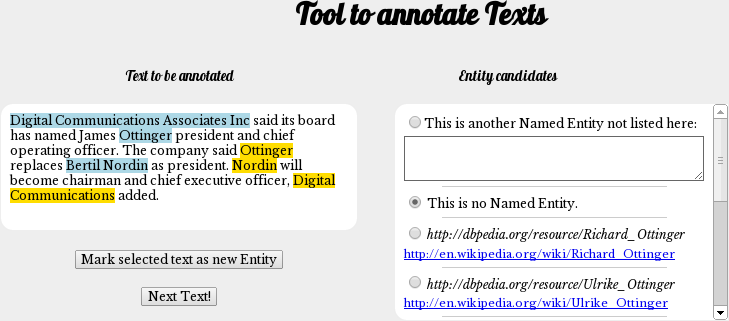
\includegraphics[width=\linewidth]{part_02/benchmarking/LREC_N3NIFNERNED/qrtool.png}
\caption{GUI of our annotation tool.}
\label{n3:fig:qrtool}
\end{figure}


\subsection{RSS-500}

This corpus has been created using a dataset comprising a list of 1,457 RSS feeds as compiled in~\cite{GOLDHAHN12.327}.
The list includes all major worldwide newspapers and a wide range of topics, e.g., \emph{World}, \emph{U.S.}, \emph{Business}, \emph{Science} etc.
The RSS list has been compiled using a 76-hour crawl, which resulted in a corpus of about 11.7 million sentences.
A subset of this corpus has been created by randomly selecting 1\% of the contained sentences.
 
Finally, one researcher annotated 500 randomly chosen sentences manually.
These sentences were a subset of those which contained a natural language representation of a formal relation, like ``\ldots, who was born in\ldots '' for \texttt{dbo:birthPlace}, cf.~\cite{conf/ekaw/GerberN12}.
The relations had to occur more than 5 times in the 1\% corpus. % with DBpedia URIs.
In case the mentioned entity is not contained in a new URI has been generated.
This corpus has been used for evaluation purposes in~\cite{GER+13}.

\section{Using NIF for publishing corpora}
\label{n3:NIF}



\begin{figure}[htb!]
\begin{lstlisting}[label=n3:TripleExampleNIF,caption=Example of the resulting N3-triples.]{TripleExampleNIF}
@prefix nif:     <http://persistence.uni-leipzig.org/nlp2rdf/ontologies/nif-core#> .
@prefix itsrdf:  <http://www.w3.org/2005/11/its/rdf#> .
@prefix xsd:     <http://www.w3.org/2001/XMLSchema#> .

<http://aksw.org/N3/Reuters-128/1#char=0,337>
      a       nif:String , nif:Context , nif:RFC5147String ;
      nif:beginIndex "0"^^xsd:int ;
      nif:endIndex "337"^^xsd:int ;
      nif:isString "Key Tronic corp said it has received contracts..."@en ;
      nif:sourceUrl <http://www.research.att.com/~lewis/Reuters-21578/15003> .

<http://aksw.org/N3/Reuters-128/1#char=0,15>
      a       nif:String , nif:RFC5147String ;
      nif:anchorOf "Key Tronic corp"^^xsd:string ;
      nif:beginIndex "0"^^xsd:int ;
      nif:endIndex "15"^^xsd:int ;
      nif:referenceContext  <http://aksw.org/N3/Reuters-128/1#char=0,337> ;
      itsrdf:taIdentRef <http://dbpedia.org/resource/Key_Tronic> ;
      itsrdf:taSource "DBpedia_en_3.9"^^xsd:string .
\end{lstlisting}
\end{figure}




For publishing our datasets, we choose NIF because it is a \ac{RDF}-based Linked Data serialization.
NIF provides different advantages, e.g., \emph{interoperability by standardization}~\cite{ISWC2013NIF} or \emph{query-ability}.
The \emph{NIF-standard} assigns each document an URI as starting point and generates another \ac{LD}  resource per NE.
Each document is a resource of type \texttt{nif:Context} and its content is the literal of its \texttt{nif:isString} predicate. 
Where possible, we added the source from which we got the document using the \texttt{nif:sourceUrl} predicate.
%where possible, the source from which the document was added used...predicate....
Every NE is an own resource with a newly generated URI pointing to the original document via the \texttt{nif:referenceContext} predicate.
Additionally, the begin (\texttt{nif:beginIndex}) and end position (\texttt{nif:endIndex}) as well as the disambiguated URI (\texttt{itsrdf:taIdentRef}) and the respective \ac{KB}  (\texttt{itsrdf:taSource}) are stored.
In contrast to Steinmetz~et~al.~\cite{NEDstatBench}, mentioning the source of annotation serves as a more useful semantic background and is thus more valuable for further research.
For instance, NIF document as depicted in Listing~\ref{n3:TripleExampleNIF} has been transformed from the document from Listing~\ref{n3:TripleExample}.

%\todo[inline]{syntax coloring is nice :) Micha: ich such mal ein paar schoene Farben ;)}
\begin{figure}[htb!]
\begin{lstlisting}[label=n3:TripleExample,caption=Example input text.]{TripleExample}
Source = Reuters-21578
ID     = 15003
Text   = Key Tronic corp said it has received contracts...
\end{lstlisting}
\end{figure}




The second advantage of using a corpus in NIF is that it is searchable using SPARQL.
When the corpus is loaded in a Triple Store (e.g., Virtuoso\footnote{\url{http://sourceforge.net/projects/virtuoso/}}) one can easily find all NEs by posing a simple SPARQL query, as depicted in Listing~\ref{n3:SPARQL1}.
\begin{figure}[htb!]
\begin{lstlisting}[label=n3:SPARQL1,caption=SPARQL query to get all NEs.]{SPARQL1}
Select ?namedEntity {[] itsrdf:taIdentRef ?namedEntity }
\end{lstlisting}
\end{figure}
\section{Conclusion}

Here, we presented three different corpora.
They can be used for \ac{NER}  and \ac{NED}  benchmarks as well as algorithm tuning.
We compared these corpora with two already known datasets and showed the advantages of our datasets.
The usability of these corpora for \ac{NED}  benchmark has been proven in \cite{agdistis_iswc,GER+13}.
Especially, we aim at providing a structured and standardized language resource for unstructured texts, enabling semantic querying.
Our datasets link \ac{NLP}  algorithms to the Semantic Web by leveraging the power of NIF and \ac{LD} .

In the future, the enlargement of the corpora and the improvement of their quality through the community are major issues that need to be worked on. 
Furthermore, converting more existing datasets to NIF and re-bundle them in order to provide even more insightful NER and NED benchmarks is the next step of research in this area.

